% =============================================================================
% File        : poster.tex
% Project     : The Knowledge Lifecycle of Large Language Models
% Purpose     : A0 portrait conference poster, carrying the five lifecycle
%               colors used by the paper, the deck, the repository, the demo.
% Authors     : Amey Thakur, Sarvesh Talele
% Repository  : https://github.com/Amey-Thakur/LLM-KNOWLEDGE-LIFECYCLE
% License     : CC BY 4.0
% =============================================================================
%
% GEOMETRY. A0 portrait is 84.1 x 118.9 cm; with the class margin the usable
% width is about 81 cm.
%
% TYPE SIZE. Every figure is drawn in arbitrary units and wrapped in
% \resizebox{\linewidth}{!}{...}. That fixes the width exactly, but it also
% scales the type inside, so a figure whose natural width is far from its
% container renders its labels at a different size from the body text. Earlier
% drafts read as a page assembled from several documents for that reason. Each
% figure below is therefore drawn at a natural width of (container / 1.4), so
% every one lands on the same 1.4x scale and every label is the same size:
% about 35 pt against 25 pt body text, which is the right relationship for
% something read standing up.
%
%   full width  81.0 cm  ->  58.0 units      0.34 column  25.5 cm  ->  18.2
%   0.58 column 45.5 cm  ->  32.5 units      0.32 column  24.0 cm  ->  17.1
%   0.42 column 32.5 cm  ->  23.2 units
%
% NO OVERLAP. Free text placed at hand-picked tikz coordinates is where words
% collide, because the width of a label is not known when its neighbor is
% positioned. Two defenses are used. Anything that is really a list, a callout
% or a code sample is built from LaTeX boxes, which cannot overlap by
% construction. Where geometry genuinely is needed, every text node is given an
% explicit text width and the clearance to its neighbor is worked out from the
% average character advance of about 0.45 units at body size.
%
% VERTICAL BUDGET. About 112 cm of height after margins. tikzposter silently
% drops anything that runs past the bottom of the page, so content that does not
% fit disappears without an error. Two earlier drafts lost their footer that way.
%
% COLUMN BALANCE. Blocks in a row are independent, so a short column leaves
% visible dead space beside a long one. The coverage statistic sits in the left
% column of row 1, and the limits note closes the right column of row 3,
% specifically so the two rows come out level.
%
% READING ORDER runs down the page, not down each column: problem, framework,
% evidence, then the contributions and how to check them.
%
% hyperref is deliberately absent: tikzposter applies its theme inside a group,
% and hyperref fails there whether loaded before or after \usetheme. At A0 a
% clickable link buys nothing, so URLs are plain text.

\documentclass[25pt, a0paper, portrait, blockverticalspace=14mm, colspace=18mm,
               subcolspace=8mm]{tikzposter}

\usepackage{amsmath}
\usepackage{amssymb}
\usepackage{tikz}
\usetikzlibrary{arrows.meta, positioning, calc, decorations.pathreplacing}

% Sans throughout. The figures are drawn in sans, and an earlier draft left the
% body in the default serif, so the page read as two documents pasted together.
\renewcommand{\familydefault}{\sfdefault}

% --- the five lifecycle colors, identical across every surface ---------------
\definecolor{acquire} {HTML}{4A7FD4}
\definecolor{store}   {HTML}{2A9D8F}
\definecolor{retrieve}{HTML}{E08A2E}
\definecolor{update}  {HTML}{D05353}
\definecolor{forget}  {HTML}{8F5FB8}
\definecolor{ink}     {HTML}{1A1A1C}
% Darkened from the screen palette: at A0 a light gray secondary reads as faint
% rather than as quiet, and the poster is printed, not backlit.
\definecolor{muted}   {HTML}{4A4A55}
\definecolor{hairline}{HTML}{C8CAD2}
\definecolor{ok}      {HTML}{2E7D32}
\definecolor{panel}   {HTML}{F4F4F7}

\usetheme{Default}
\usebackgroundstyle{Empty}
\usetitlestyle{Empty}

% Minimal is the built-in style that rules under the block title. A custom style
% was tried first and broke the build: its rule dereferences the blocktitle
% node, which does not exist for a block with an empty title.
\useblockstyle{Minimal}

\colorlet{backgroundcolor}{white}
\colorlet{framecolor}{acquire}
\colorlet{blocktitlebgcolor}{white}
\colorlet{blocktitlefgcolor}{ink}
\colorlet{blockbodybgcolor}{white}
\colorlet{blockbodyfgcolor}{ink}

% -----------------------------------------------------------------------------
% The identity band. Drawn 58 units wide so it scales like every figure.
% -----------------------------------------------------------------------------
\newcommand{\stageband}[1]{%
  \resizebox{\linewidth}{!}{%
    \begin{tikzpicture}
      \foreach \c [count=\i from 0] in {acquire, store, retrieve, update, forget}
        \fill[\c] (\i*11.6, 0) rectangle (\i*11.6 + 11.6, #1);
    \end{tikzpicture}}%
}

% The band below the authors also names the stages, so it divides the header
% from the content and teaches the framework in the same stroke. Each cell is
% 11.6 units and the longest name, RETRIEVE, is about 4.0 units, so no name can
% reach its neighbor.
\newcommand{\stagebandnamed}{%
  \resizebox{\linewidth}{!}{%
    
\begin{tikzpicture}
      \foreach \c/\n [count=\i from 0] in
        {acquire/ACQUIRE, store/STORE, retrieve/RETRIEVE, update/UPDATE, forget/FORGET}
        {\fill[\c] (\i*11.6, 0) rectangle (\i*11.6 + 11.6, 1.9);
         \node[text=white, font=\bfseries] at (\i*11.6 + 5.8, 0.95) {\n};}
    \end{tikzpicture}}%
}

% -----------------------------------------------------------------------------
% A callout: an accent rule, a tinted panel, and text that wraps inside it.
% Built from a self-sizing node rather than fixed coordinates, so the panel is
% always exactly as tall as its content and the text can never spill out of it.
% The 10 mm inner padding clears the 6 mm accent rule by 4 mm.
% -----------------------------------------------------------------------------
\newlength{\calloutwidth}
\newcommand{\callout}[2]{%  #1 = accent color, #2 = content
  \setlength{\calloutwidth}{\dimexpr\linewidth-20mm\relax}%
  \noindent\begin{tikzpicture}
    \node[fill=panel, text width=\calloutwidth, inner sep=10mm,
          align=left, anchor=north west] (c) at (0,0) {#2};
    \fill[#1] (c.south west) rectangle ([xshift=6mm]c.north west);
  \end{tikzpicture}%
}

\title{The Knowledge Lifecycle of Large Language Models}
\author{Amey Thakur \quad Sarvesh Talele}
\institute{Independent Research}

\settitle{
  \centering
  \stageband{0.9}
  \vspace{11mm}

  % Scaled to the measure rather than set at a fixed point size. This is what
  % keeps the title on one line: the size follows from the width instead of the
  % line breaking wherever a guessed size happens to run out.
  \resizebox{\linewidth}{!}{\bfseries\color{ink}%
    The Knowledge Lifecycle of Large Language Models}
  \vspace{9mm}

  {\fontsize{40}{50}\selectfont\color{muted}
   A model holds two memories. When they disagree, training usually wins.\par}
  \vspace{12mm}

  % Two equal bays with a fixed gutter, so the author strip is symmetric about
  % the center of the page whatever the two names measure.
  \begin{minipage}[c]{0.44\linewidth}\raggedleft
    \begin{minipage}[c]{3.8cm}
\includegraphics[width=3.6cm]{amey-circle.png}\end{minipage}%
    \hspace{6mm}%
    \begin{minipage}[c]{16cm}\raggedright
      {\fontsize{36}{42}\selectfont\bfseries\color{ink} Amey Thakur\par}
      \vspace{1mm}
      {\fontsize{26}{32}\selectfont\color{muted} Toronto, Canada\par}
      {\fontsize{24}{30}\selectfont\color{muted} ORCID 0000-0001-5644-1575\par}
    \end{minipage}
  \end{minipage}%
  \hspace{0.04\linewidth}%
  \begin{minipage}[c]{0.44\linewidth}\raggedright
    \begin{minipage}[c]{3.8cm}
\includegraphics[width=3.6cm]{sarvesh-circle.png}\end{minipage}%
    \hspace{6mm}%
    \begin{minipage}[c]{16cm}\raggedright
      {\fontsize{36}{42}\selectfont\bfseries\color{ink} Sarvesh Talele\par}
      \vspace{1mm}
      {\fontsize{26}{32}\selectfont\color{muted} Mumbai, India\par}
      {\fontsize{24}{30}\selectfont\color{muted} ORCID 0009-0002-0818-461X\par}
    \end{minipage}
  \end{minipage}
  \vspace{12mm}

  \stagebandnamed
  \vspace{2mm}
}

\begin{document}

\maketitle[width=\textwidth]

% =============================================================================
% ROW 1  |  the problem, and the framework that answers it
% =============================================================================
\begin{columns}
\column{0.42}
\colorlet{framecolor}{update}
\block{The problem}{
  How a language model handles a fact is studied by \textbf{five separate
  communities} that rarely cite one another.
  \vspace{8mm}

  % A tabular, not a tikzpicture: the swatch and its label sit in separate
  % cells, so no amount of text can push one into the other.
  \noindent
  \begin{tabular}{@{}l@{\hspace{8mm}}l@{}}
    \textcolor{acquire} {\rule[-1mm]{16mm}{10mm}} & retrieval-augmented generation \\[6mm]
    \textcolor{store}   {\rule[-1mm]{16mm}{10mm}} & knowledge editing              \\[6mm]
    \textcolor{retrieve}{\rule[-1mm]{16mm}{10mm}} & continual learning             \\[6mm]
    \textcolor{update}  {\rule[-1mm]{16mm}{10mm}} & context engineering            \\[6mm]
    \textcolor{forget}  {\rule[-1mm]{16mm}{10mm}} & agent memory                   \\
  \end{tabular}
  \vspace{9mm}

  Each has its own benchmarks, and each passes them. A system can pass
  \textbf{all five} and still fail, because nothing tests what happens
  \textbf{between} them.
  \vspace{9mm}

  \callout{acquire}{Across \textbf{20 representative papers}, the median work
    covers \textbf{two} of the five stages. The boundaries are where deployment
    breaks.}
}

\column{0.58}
\colorlet{framecolor}{acquire}
\block{The framework}{
  A fact passes through five stages. Naming them as one lifecycle is what makes
  the boundaries between them visible.
  \vspace{8mm}

  % Natural width 32.3 units against a 45.5 cm column: the 1.4x figure scale.
  % Boxes are 5.5 wide on a 6.7 pitch. Each caption is confined to a 5.5 unit
  % text width, so the 1.2 unit gutter between boxes is never encroached on.
  \resizebox{\linewidth}{!}{%
  \begin{tikzpicture}[
    stage/.style={rounded corners=3pt, minimum width=5.5cm, minimum height=3.0cm,
                  text=white, font=\bfseries, align=center},
    cap/.style={text=muted, font=\small, text width=5.5cm, align=center},
    flow/.style={-{Stealth[length=5mm, width=3.5mm]}, line width=2.5pt, muted}
  ]
    \node[stage, fill=acquire]  (a) at (0,0)    {Acquire};
    \node[stage, fill=store]    (s) at (6.7,0)  {Store};
    \node[stage, fill=retrieve] (r) at (13.4,0) {Retrieve};
    \node[stage, fill=update]   (u) at (20.1,0) {Update};
    \node[stage, fill=forget]   (f) at (26.8,0) {Forget};

    \draw[flow] (a) -- (s);
    \draw[flow] (s) -- (r);
    \draw[flow] (r) -- (u);
    \draw[flow] (u) -- (f);

    \node[cap, below=4mm of a] {training};
    \node[cap, below=4mm of s] {weights};
    \node[cap, below=4mm of r] {attention};
    \node[cap, below=4mm of u] {editing};
    \node[cap, below=4mm of f] {unlearning};

    % The conflict spans two stages, so it is a brace beneath them rather than a
    % label on the arrow between them, where it collided with the Update box.
    % Captions bottom out near y = -2.8; the brace sits at -3.8 and its label at
    % -5.1, so neither can touch them.
    \draw[update, line width=2.5pt, decorate,
          decoration={brace, mirror, amplitude=5mm}]
      (10.65, -3.8) -- (22.85, -3.8);
    \node[text=update, font=\bfseries] at (16.75, -5.1) {conflict};
    \useasboundingbox (-3.0, -6.0) rectangle (29.6, 1.8);
  \end{tikzpicture}}
  \vspace{9mm}

  The failure below sits between \textcolor{retrieve}{\textbf{Retrieve}} and
  \textcolor{update}{\textbf{Update}}: the document arrives, and nothing tells
  the model which copy of the fact to trust. That boundary belongs to neither
  field beside it, which is why nobody tests it.
}
\end{columns}

% =============================================================================
% ROW 2  |  the finding, full width, the largest figure on the page
% =============================================================================
\colorlet{framecolor}{update}
\block{The finding}{
  Vioxx was withdrawn worldwide in September 2004 for raising the risk of heart
  attack and stroke. Put that withdrawal notice \textbf{directly into GPT-2's
  prompt}, then ask whether the drug is safe to prescribe.
  \vspace{8mm}

  % Natural width 58 units against the 81 cm measure: the 1.4x figure scale.
  % Lane plan, in units, with every reserved span written down so that no two
  % pieces of text can be placed on top of one another:
  %   row label   0.0 - 10.5   longest is ``withdrawn'' at 6.6
  %   panel A     12.0 - 33.0  header 8.1 wide, bar at most 11.3, value 3.0
  %   panel B     35.0 - 56.0  header 13.1 wide, bar at most 12.8, value 3.0
  % Bar scale is 0.30 units per percentage point.
  \resizebox{\linewidth}{!}{%
  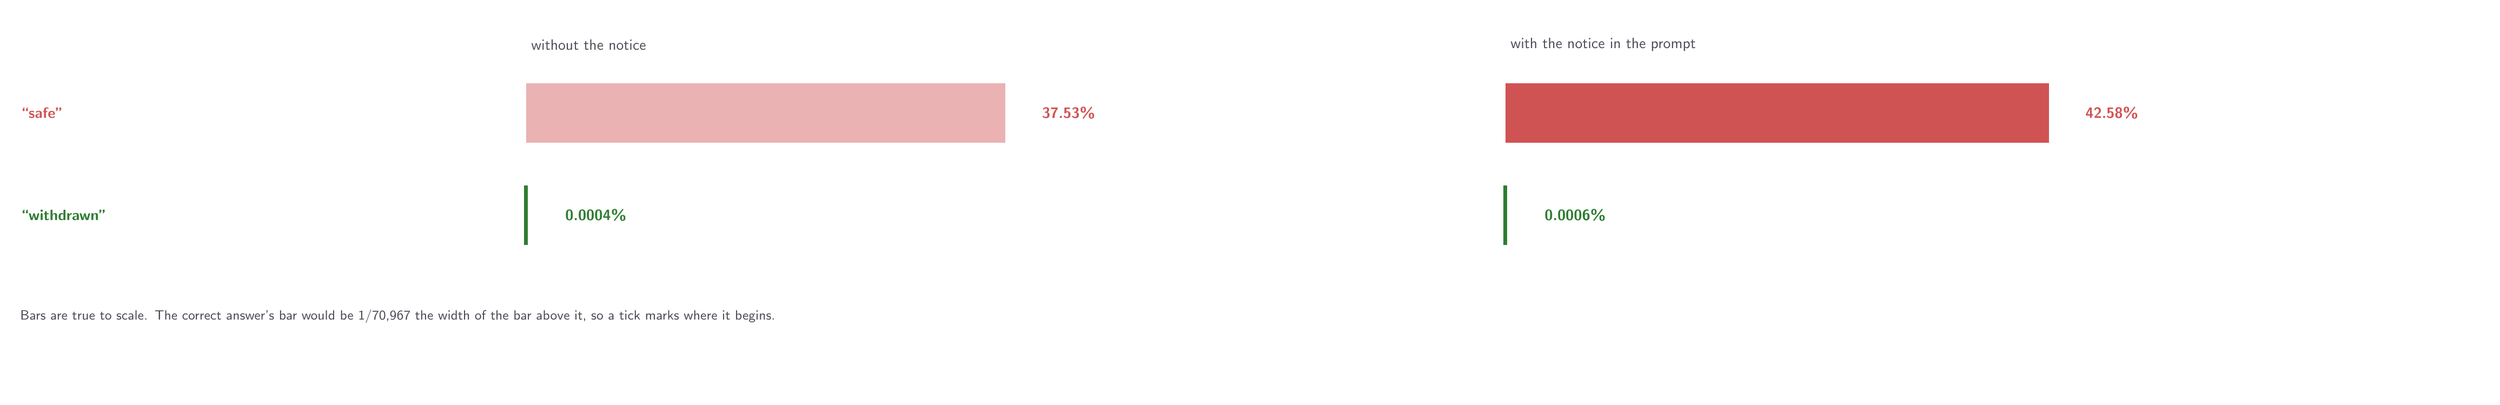
\begin{tikzpicture}
    \node[anchor=west, text=muted, text width=20cm] at (12, 5.7)
      {without the notice};
    \node[anchor=west, text=muted, text width=21cm] at (35, 5.7)
      {with the notice in the prompt};

    % --- the model's answer, wrong ------------------------------------------
    \node[anchor=west, font=\bfseries, text=update, text width=10.5cm] at (0, 4.1)
      {``safe''};
    \fill[update!45] (12, 3.4) rectangle (23.26, 4.8);
    \node[anchor=west, font=\bfseries, text=update] at (24.0, 4.1) {37.53\%};
    \fill[update]    (35, 3.4) rectangle (47.77, 4.8);
    \node[anchor=west, font=\bfseries, text=update] at (48.5, 4.1) {42.58\%};

    % --- the correct answer --------------------------------------------------
    % At this scale the correct answer's bar is 1/70,967 the width of the one
    % above it, far below a printed pixel, so a tick marks its origin. Drawing a
    % visible sliver would overstate the result by three orders of magnitude.
    % The two values sit beside their own ticks rather than under the values
    % above, so that neither number can be read against the wrong bar.
    \node[anchor=west, font=\bfseries, text=ok, text width=10.5cm] at (0, 1.7)
      {``withdrawn''};
    \draw[ok, line width=2.5pt] (12, 1.0) -- (12, 2.4);
    \node[anchor=west, font=\bfseries, text=ok] at (12.8, 1.7) {0.0004\%};
    \draw[ok, line width=2.5pt] (35, 1.0) -- (35, 2.4);
    \node[anchor=west, font=\bfseries, text=ok] at (35.8, 1.7) {0.0006\%};

    \node[anchor=north west, text=muted, font=\small, text width=56cm, align=left]
      at (0, -0.4)
      {Bars are true to scale. The correct answer's bar would be 1/70{,}967 the
       width of the bar above it, so a tick marks where it begins.};
    \useasboundingbox (0, -2.4) rectangle (58, 6.4);
  \end{tikzpicture}}
  \vspace{9mm}

  \callout{update}{%
    {\Large\bfseries The correction is sitting in the prompt, and confidence
     that the drug is safe \textcolor{update}{goes up}.\par}
    \vspace{6mm}
    {\color{muted}Retrieval worked. What failed is the step after it, where the
     model has to decide which of its two memories to believe.\par}}
}

% =============================================================================
% ROW 3  |  the two contributions, and how to check them
% =============================================================================
\begin{columns}
\column{0.34}
\colorlet{framecolor}{retrieve}
\block{A metric}{
  \textbf{Lifecycle Desynchronization} is the surprisal of the \textbf{correct}
  answer while the corrective document is present:
  \vspace{5mm}
  \begin{equation*}
    \widehat{\mathcal{D}}_{sync}
      = -\ln P\!\left(y^{*} \mid q,\, \theta_{stale},\, \mathcal{M}_{now}\right)
  \end{equation*}
  \vspace{3mm}

  It is read in nats: $n$ nats means probability $e^{-n}$. Past \textbf{9.2} the
  correct answer is below one chance in ten thousand.
  \vspace{9mm}

  % Natural width 17.2 units against a 25.5 cm column: the 1.4x figure scale.
  % 1.214 units per nat. Tick labels are about 1.1 units wide and the closest
  % pair, 9.2 and the 12.05 marker, are 3.5 units apart.
  \resizebox{\linewidth}{!}{%
  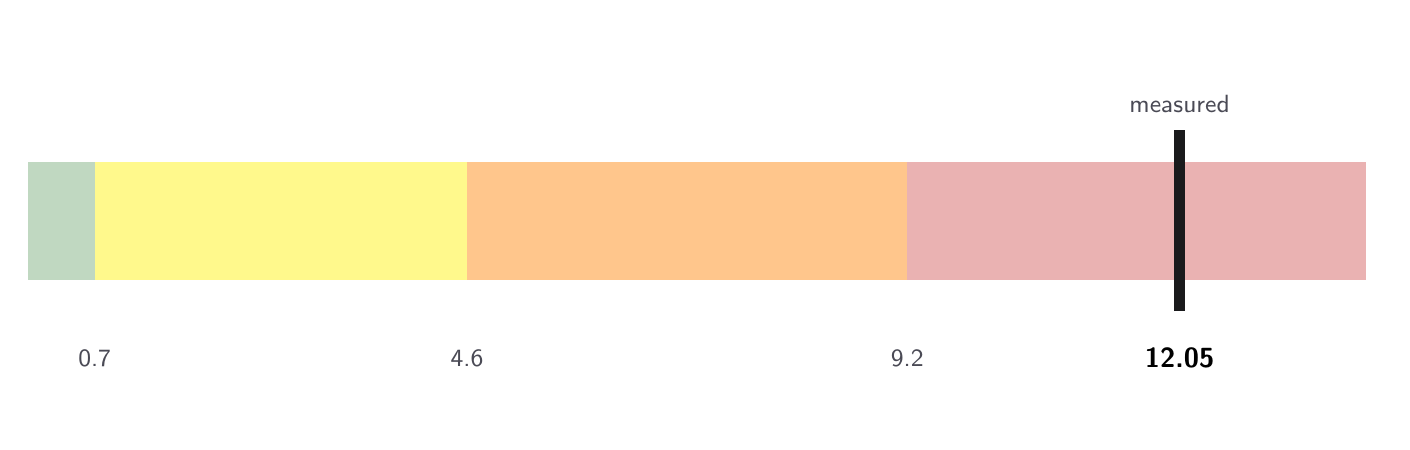
\begin{tikzpicture}
    \fill[ok!30]     (0,     0) rectangle (0.85,  1.5);
    \fill[yellow!45] (0.85,  0) rectangle (5.58,  1.5);
    \fill[orange!45] (5.58,  0) rectangle (11.17, 1.5);
    \fill[update!45] (11.17, 0) rectangle (17.00, 1.5);

    \draw[ink, line width=4pt] (14.63, -0.4) -- (14.63, 1.9);
    \node[anchor=south, text=muted, font=\small] at (14.63, 2.0) {measured};

    \node[text=muted, font=\small] at (0.85,  -1.0) {0.7};
    \node[text=muted, font=\small] at (5.58,  -1.0) {4.6};
    \node[text=muted, font=\small] at (11.17, -1.0) {9.2};
    \node[font=\bfseries]          at (14.63, -1.0) {12.05};
    \useasboundingbox (0, -1.8) rectangle (17.2, 3.2);
  \end{tikzpicture}}
  \vspace{9mm}

  A companion number, \textbf{context influence}, asks whether the document
  moved the model at all. Here it is \textbf{0.033} nats: the evidence is
  present, and \textbf{inert}.
}

\column{0.34}
\colorlet{framecolor}{store}
\block{An architecture}{
  Storage records \textbf{what} is true but never \textbf{when} it was learned,
  so nothing lets the model prefer fresh evidence over a confident old memory.
  \vspace{9mm}

  % Natural width 18.0 units against a 25.5 cm column: the 1.4x figure scale.
  % Slots are 5.0 wide on a 6.5 pitch, so the gutter is 1.5 and each label is
  % held inside a 4.2 unit text width, well clear of it.
  \resizebox{\linewidth}{!}{%
  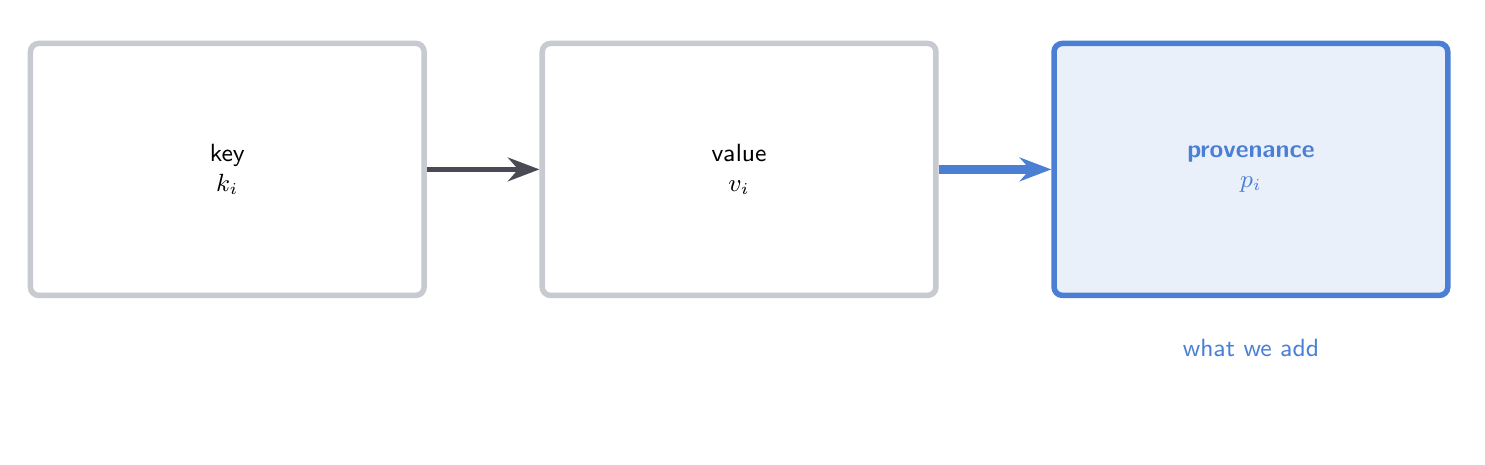
\begin{tikzpicture}[
    slot/.style={rounded corners=3pt, minimum width=5.0cm, minimum height=3.2cm,
                 align=center, draw=hairline, line width=2pt,
                 font=\small, text width=4.2cm}
  ]
    \node[slot] (k) at (0,0)   {key\\ $k_i$};
    \node[slot] (v) at (6.5,0) {value\\ $v_i$};
    \node[slot, draw=acquire, fill=acquire!12, text=acquire] (p) at (13.0,0)
      {\textbf{provenance}\\ $p_i$};

    \draw[-{Stealth[length=4mm]}, muted,   line width=2pt] (k) -- (v);
    \draw[-{Stealth[length=4mm]}, acquire, line width=3pt] (v) -- (p);
    \node[below=4mm of p, text=acquire, font=\small, text width=5.0cm,
          align=center] {what we add};
    \useasboundingbox (-2.5, -3.4) rectangle (15.5, 1.8);
  \end{tikzpicture}}
  \vspace{9mm}

  The \textbf{Provenance Vector} attaches acquisition time to every memory slot.
  A gate reads it at inference and mutes facts that have gone stale:
  \vspace{4mm}
  \begin{equation*}
    S(\Delta\tau_i) = \sigma\!\left(\gamma - \beta\,\Delta\tau_i\right)
  \end{equation*}
  \vspace{4mm}

  \textbf{Weights are never modified}, so the specificity bottleneck that limits
  static editing does not apply. Under \textbf{0.02\%} extra parameters.
}

\column{0.32}
\colorlet{framecolor}{forget}
\block{Reproduce it}{
  Every number on this poster comes from \textbf{one deterministic script}.
  Nothing is sampled, so the digits come out identical on any machine.
  \vspace{9mm}

  \callout{forget}{\ttfamily
    pip install torch transformers\par
    \vspace{4mm}
    python dsync\_experiment.py}
  \vspace{9mm}

  It runs on \textbf{GPT-2 base}, 124M parameters: small, fully open, and with
  no instruction tuning to confound the result. A laptop is enough.
  \vspace{9mm}

  The metric is \textbf{measured}. The architecture is \textbf{proposed} and has
  not been trained.
  \vspace{9mm}

  \callout{muted}{\color{muted}One model, one fact, one prompt. The size of the
    effect is what needs replication across models, and the repository carries
    the notebook for doing it.}
}

\end{columns}

% =============================================================================
% FOOT  |  where to find the work, then the identity band closing the page
% =============================================================================
\colorlet{framecolor}{hairline}
\block{}{
  \textcolor{hairline}{\rule{\linewidth}{2pt}}
  \vspace{9mm}

  % Three bays of equal width separated by equal gutters, so the row is
  % symmetric about the center of the page by construction rather than by
  % coordinates that happen to be evenly spaced. Each bay is a heading and two
  % short lines, so the three also come out level.
  \noindent
  \begin{minipage}[t]{0.30\linewidth}\centering
    {\bfseries Paper and code}\par\vspace{3mm}
    {\small\color{muted} github.com/Amey-Thakur/\par LLM-KNOWLEDGE-LIFECYCLE\par}
  \end{minipage}\hfill
  \begin{minipage}[t]{0.30\linewidth}\centering
    {\bfseries Live demonstration}\par\vspace{3mm}
    {\small\color{muted} huggingface.co/spaces/ameythakur/\par llm-knowledge-lifecycle\par}
  \end{minipage}\hfill
  \begin{minipage}[t]{0.30\linewidth}\centering
    {\bfseries ORCID}\par\vspace{3mm}
    {\small\color{muted} Thakur 0000-0001-5644-1575\par Talele 0009-0002-0818-461X\par}
  \end{minipage}
  \vspace{9mm}

  {\centering\small\color{muted} Released under CC BY 4.0\par}
  \vspace{7mm}

  \stageband{0.9}
}

\end{document}
